\documentclass{uofsthesis-cs}
\usepackage{graphicx}
\graphicspath{ {./images/c2/}, {./images/c3/}, {./images/}}
\usepackage{amsmath}
\usepackage{amsfonts}
\usepackage{changes}
\usepackage{bm}
\definechangesauthor[name=Dave Schneider, color=red]{djs}
\definechangesauthor[name=Yujie Pei, color=green]{Yuge}
\usepackage{caption}
\usepackage{subcaption}
\usepackage{booktabs}
\usepackage{algorithmic} % package for generating algorithms
\setcounter{secnumdepth}{4}
\setcounter{tocdepth}{4}

\newcommand{\subsubsubsection}[1]{\paragraph{#1}\mbox{}\\}




\title{An Alternative Method for Characterization and Comparison of Plant Root Shapes}


\author{Yujie Pei}
\degree{\MSc}
\defencedate{Month/Year}
\department{School of Environment and Sustainability}
%\Academicunit{Master of Environment and Sustainability}



\begin{document}


% ___________________________ BEFORE THE BODY OF THESIS _______________

% baesed on https://students.usask.ca/graduate/thesis-preparation.php#ArrangementofContents

\maketitle % 1. Title Page

% 2. Permission to use and disclaimer Statement

%\abstract{}  % 3. abstract

%\acknowledgements{}  % 4. Acknowledgements

% 5. Permission to Reproduce 

%\dedication{}  % 6. Dedication

\tableofcontents % 7. Table of content

% 8. List of tables

% 9. List of figures

% 10. List of abbreviation



% 11. Body of the Thesis

% ___________________________ BODY OF THESIS _________________________

%%%%%%%%%%%%%%%%%%%%%%%%%% CHAPTER 1 %%%%%%%%%%%%%%%%%%%%%%%%%%%%%%%%%%

\chapter{Existing Morphological Descriptors for Root Systems}

  %\include{}

  
  
%%%%%%%%%%%%%%%%%%%%%%%%%% CHAPTER 2 %%%%%%%%%%%%%%%%%%%%%%%%%%%%%%%%%%

\chapter{An Alternative Mathematical Method for Shape Description}

 


    

%%%%%%%%%%%%%%%%%%%%%%%%%% CHAPTER 3 %%%%%%%%%%%%%%%%%%%%%%%%%%%%%%%%%%
  
\chapter{LRWs in Artificial Images}

  %______________ Section 1: Circle and Rectangle ______________
  
The fixed-time step Monte Carlo simulation, LRWs, has been validated
in the annulus in Appendix \ref{appendix:method_validation_annulus} by
comparing the analytical and numerical survival function. The further
validation of LRWs is to distinguish the geometries and explore their
structural features from both short and long time survival behaviours.



\section{\highlight[id=Yuge]{Circle and Rectangle}}

Given two simple convex shapes with the same area, circle and
rectangle, we are interested in how and whether their corresponding
survival curves differ from each other. For the equal-area geometries,
rectangle and circle, Eq. \ref{eq:kac_result} indicates that the
survival function of the former decays faster than the latter as the
time approaches zero.

The preliminary step of testing the research hypothesis is to generate
two black-and-white images with the same dimensions as shown in
Fig.~\ref{fig:simple_imgs}. In the binary images, circle and rectangle
have an equal number of white pixels. For simplicity, the centroid of
shapes located at the center of the image. Then, simulating LRWs in
the images and estimating survival functions by Kaplan-Meier
estimator.


 \subsection{Output Analysis}
 
   \begin{figure}
     \centering
     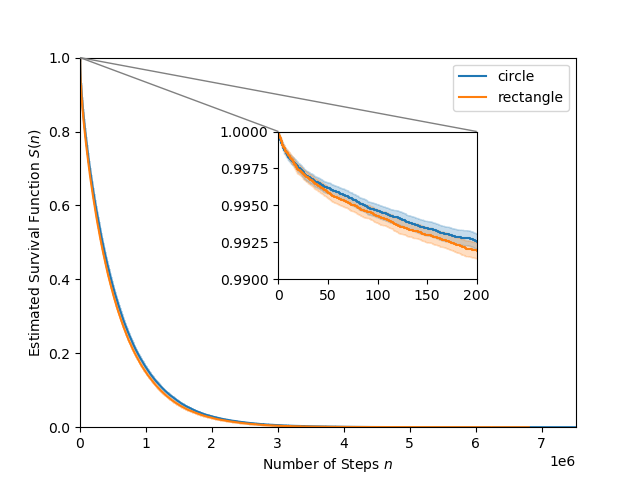
\includegraphics[width=\textwidth]{circle_rect_steps_sf.png}
     \label{fig:sf_simple_shape_steps}
     \caption{In the inset, the decay rate of the survival function for the rectangle is slightly larger than for the circle, which coincides with the theoretical result.}
   \end{figure}

  The differences between survival functions for the circle and
  rectangle are not visible. Moreover, the approximate $95\%$
  confidence intervals of the survival functions overlap. In this
  case, non-parametric statistical tests can be used to compare entire
  survival distributions and assess their dissimilarities. The logrank
  test has maximum power if the proportional hazards assumption is
  satisfied. 

   \begin{figure}
     \centering
     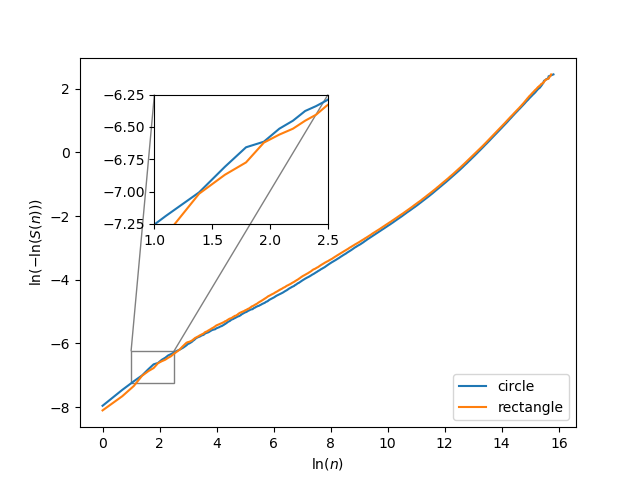
\includegraphics[width=\textwidth]{circle_rect_steps_ph.png}
     \label{fig:ph_test_simple_shapes}
     \caption{It is a graphical method for checking proportionality by looking for parallelism. As shown in the inset plot, two curves cross at some points and their shapes vary over time. Moreover, $p < 0.05$ in the non-proportional test. Thus, the survival functions for circle and rectangle do not satisfy the proportional hazard assumption.}
   \end{figure}


   \begin{table}
     \centering
     \begin{tabular}{lrr}
        \toprule
         {} &  test\_statistic &             p \\
         \midrule
         Logrank & 137.23 & 0.0 \\
         \midrule
         Tarone-Ware & 134.31 & 0.0 \\
         \midrule
         Gehan-Breslow & 123.83 & 0.0 \\
         \midrule
         Fleming-Harrington & 123.83 & 0.0 \\
         \bottomrule
     \end{tabular}
     \caption{Survival functions for circle and rectangle are statistically different since p values equal zeros.}
     \label{tab:test_simple_shape_steps}
   \end{table}



\subsection{Conclusion}


Although the proportional hazard assumption test is failed as shown in
Fig.~\ref{fig:ph_test_simple_shapes}, the weighted logrank tests
indicate that the null hypothesis should be rejected. In conclusion,
LRWs is an alternative tool to quantify and distinguish the geometries
in the $2-$ dimensional image without measuring the predefined shape
descriptors.
  


  %_______ Section 2: Complicated Branching Structures _________
  \section{Complicated Branching Structures}


   \subsection{Image Description}

     \begin{itemize}
         \item Image size: $1200 \times 1000$ pixels
         \item Surface area of shapes: $90000$ pixels
         \item Iterate the template $3, 4, 5, 6$ times to produce the targeted branching geometries labelled as $L_3, L_4, L_5, L_6$.
         \item Two groups of images labelled as $G_1, G_2$

           \begin{itemize}
             \item $G_1$: the target object $G_1 L_i$ ($i=3, 4, 5, 6$) is equidistant to the edges of an image.
             \item $G_2$: the template of $G_2 L_i$ ($i=3, 4, 5, 6$) is distinct from $G_1$ (thickness and aspect ratio). 
           \end{itemize}
           
     \end{itemize}



   \subsection{Output Analysis}


     \subsubsection{$S(n)$}



       \subsubsubsection{Estimated Survival Curves}

     
       \begin{figure}
        \centering
        
        \begin{subfigure}[b]{0.45\textwidth}
          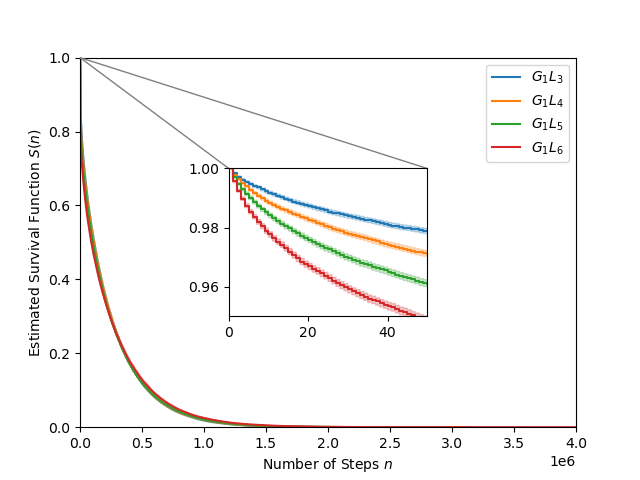
\includegraphics[width=\textwidth]{G_1_steps_sf.png}
          \caption{}
          \label{fig:sf_g1_branch_steps}
        \end{subfigure}
        \hfill
        \begin{subfigure}[b]{0.45\textwidth}
          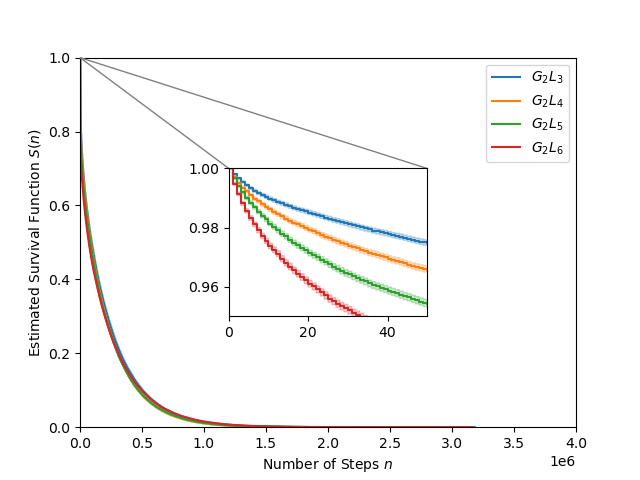
\includegraphics[width=\textwidth]{G_2_steps_sf.png}
          \caption{}
          \label{fig:sf_g2_branch_steps}
        \end{subfigure}

        \caption{}
        \label{fig:sf_branch_steps}

      \end{figure}



       \subsubsubsection{Non-Parametric Statistical Tests}

       
      \begin{table}
        \centering
        \begin{tabular}{llrrrr}
          \toprule
                       &             &         &  p &    &     \\
          \cmidrule{3-6}
                       &             & Logrank & TW & GB & FH  \\
          \midrule
          $G_1$ $L_3$  & $G_1$ $L_4$  &  0.4393 &  0.0285 &  0.0005 &  0.0005     \\
                       & $G_1$ $L_5$  & 0.0 & 0.0 & 0.0 & 0.0    \\
                       & $G_1$ $L_6$  & 0.0 & 0.0 & 0.0 & 0.0      \\
          $G_1$ $L_4$  & $G_1$ $L_5$  & 0.0007 & 0.0 & 0.0 & 0.0      \\
                       & $G_1$ $L_6$  & 0.0002 & 0.0 & 0.0 & 0.0       \\
          $G_1$ $L_5$   & $G_1$ $L_6$ & 0.7223 &  0.0 & 0.0 & 0.0      \\
          \bottomrule
        \end{tabular}
        \label{tab:g1_ingroup_tests_steps}
        \caption{}
      \end{table}


      \begin{table}
        \centering
        \begin{tabular}{llrrrr}
          \toprule
                       &             &         &  p &    &     \\
          \cmidrule{3-6}
                       &             & Logrank & TW & GB & FH  \\
          \midrule
          $G_2$ $L_3$  & $G_2$ $L_4$  &  0.0 &  0.0 &  0.0 &  0.0     \\
                       & $G_2$ $L_5$  & 0.0 & 0.0 & 0.0 & 0.0    \\
                       & $G_2$ $L_6$  & 0.0 & 0.0 & 0.0 & 0.0      \\
          $G_2$ $L_4$  & $G_2$ $L_5$  & 0.0016 & 0.0 & 0.0 & 0.0      \\
                       & $G_2$ $L_6$  & 0.0004 & 0.0 & 0.0 & 0.0       \\
          $G_2$ $L_5$   & $G_2$ $L_6$ & 0.7199 &  0.0 & 0.0 & 0.0      \\
          \bottomrule
        \end{tabular}
        \label{tab:g2_ingroup_tests_steps}
        \caption{}
      \end{table}



       \subsubsubsection{Mesurement of Dissimilarities for $S(n)$}
      

      \begin{figure}
        \centering
        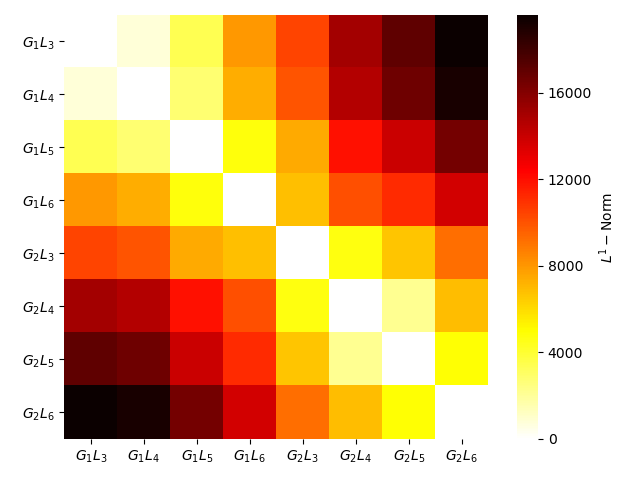
\includegraphics[width=\textwidth]{heatmap_ai_steps_l1.png}
        \caption{}
        \label{fig:heatmap_ai_steps_l1}
      \end{figure}

      
      \begin{figure}[h!]
        \centering
        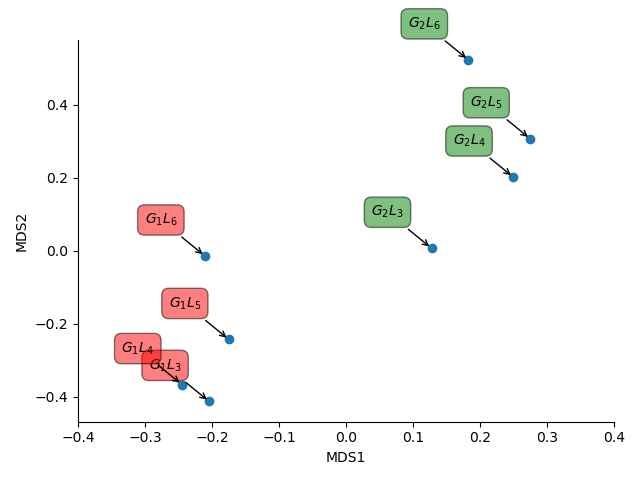
\includegraphics[width=\textwidth]{MDS_ai_steps_l1.png}
        \caption{}
        \label{fig:MDS_ai_steps_l1}
      \end{figure}
      


      
      \subsubsubsection{Visualize $S(n)$}

       \begin{figure}
         \centering
         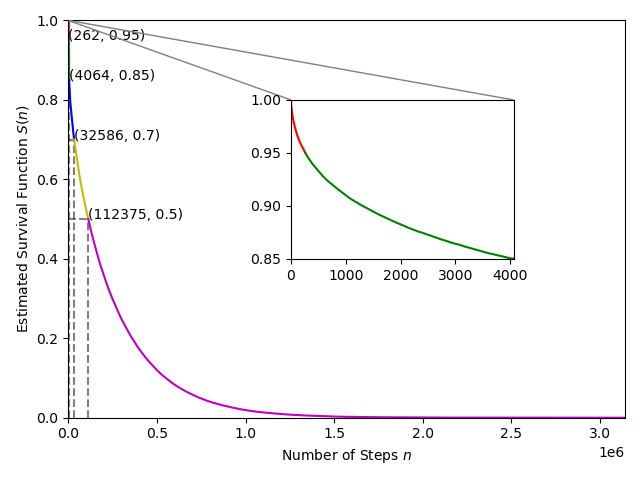
\includegraphics[width=\textwidth]{steps_seg_curve_G_1_L_3.png}
         \caption{}
         \label{fig:steps_seg_curve_G_1_L_3}
      \end{figure}



       \begin{figure}
         \centering
         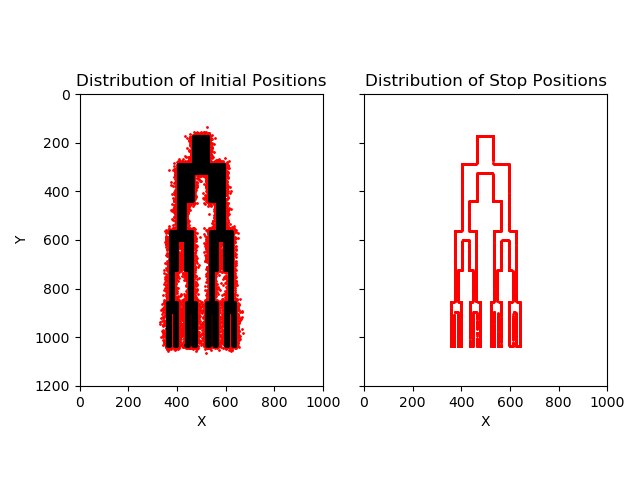
\includegraphics[width=\textwidth]{G_1_L_3_steps_red_initial_pos_distribution.png}
         \caption{}
         \label{fig:G_1_L_3_steps_red_initial_pos_distribution}
       \end{figure}



       \begin{figure}
         \centering
         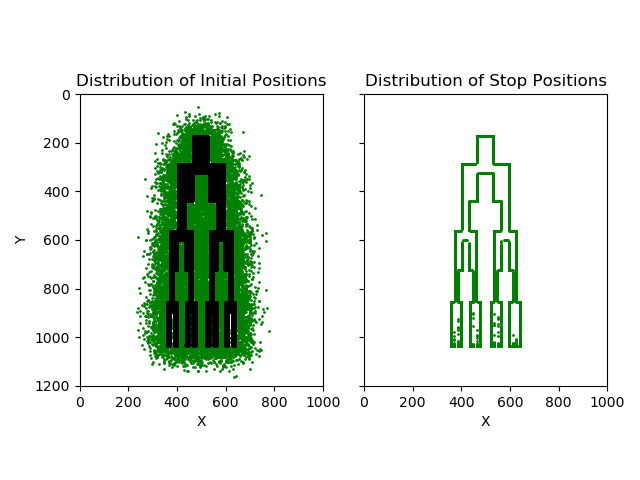
\includegraphics[width=\textwidth]{G_1_L_3_steps_green_initial_pos_distribution.png}
         \caption{}
         \label{fig:G_1_L_3_steps_green_initial_pos_distribution}
       \end{figure}


       \begin{figure}
         \centering
         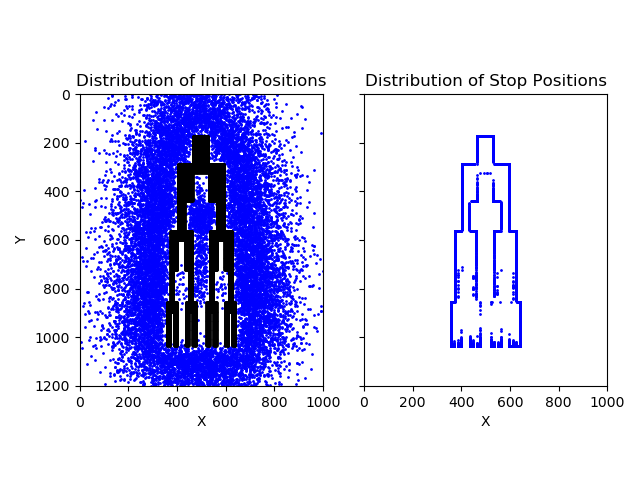
\includegraphics[width=\textwidth]{G_1_L_3_steps_blue_initial_pos_distribution.png}
         \caption{}
         \label{fig:G_1_L_3_steps_blue_initial_pos_distribution}
       \end{figure}
       

       \begin{figure}
         \centering
         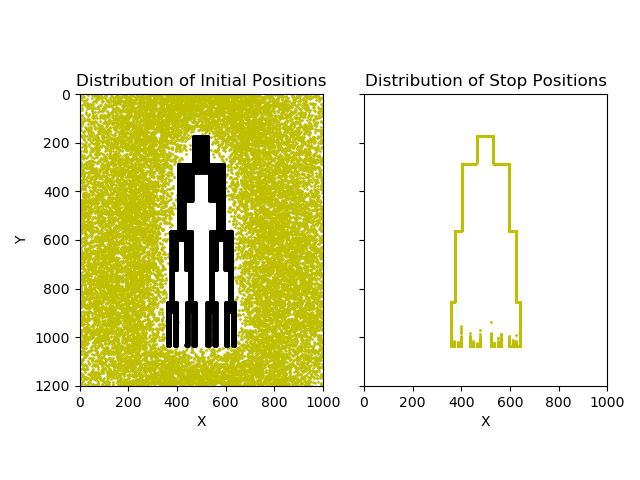
\includegraphics[width=\textwidth]{G_1_L_3_steps_y_initial_pos_distribution.png}
         \caption{}
         \label{fig:G_1_L_3_steps_y_initial_pos_distribution}
       \end{figure}


       \begin{figure}
         \centering
         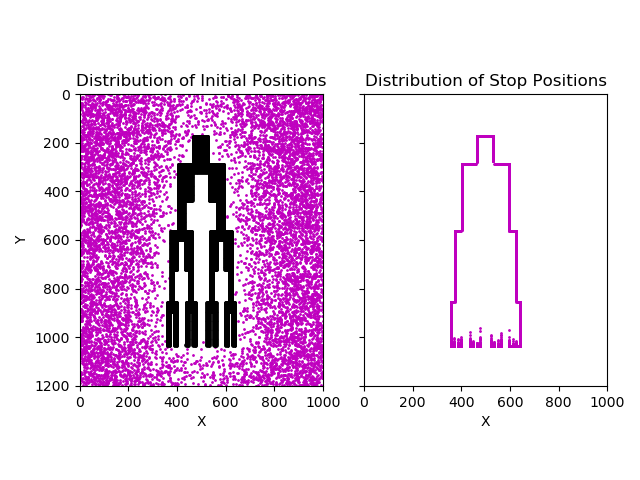
\includegraphics[width=\textwidth]{G_1_L_3_steps_m_initial_pos_distribution.png}
         \caption{}
         \label{fig:G_1_L_3_steps_m_initial_pos_distribution}
       \end{figure}


























      

      %____________________________________________________________



       \newpage

       
      \subsubsection{$S(d)$}



      \begin{figure}
        \centering
        
        \begin{subfigure}[b]{0.45\textwidth}
          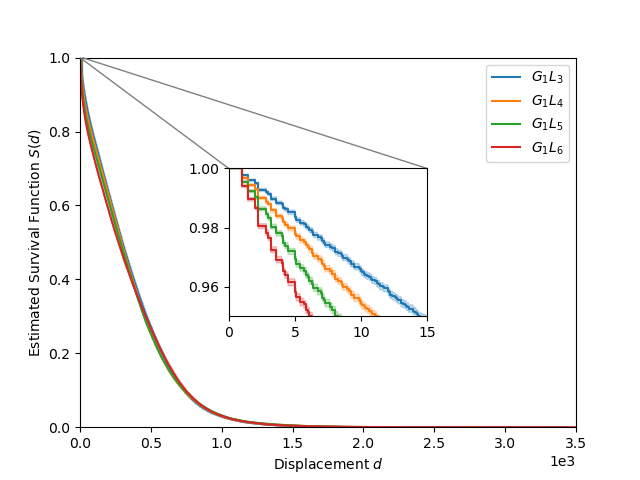
\includegraphics[width=\textwidth]{G_1_unwrap_disp_sf.png}
          \caption{}
          \label{fig:sf_g1_branch_disp}
        \end{subfigure}
        \hfill
        \begin{subfigure}[b]{0.45\textwidth}
          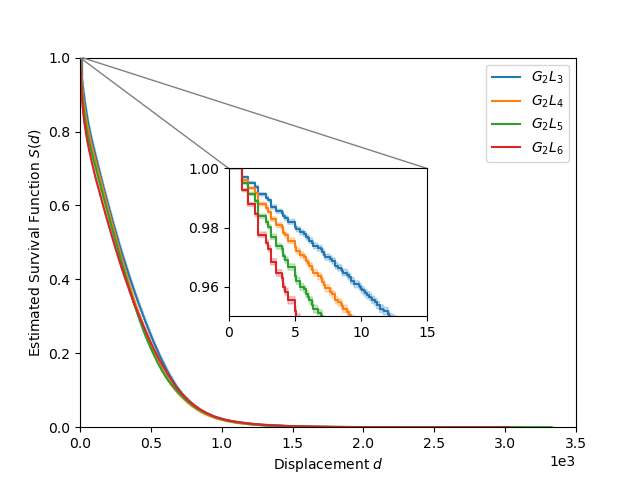
\includegraphics[width=\textwidth]{G_2_unwrap_disp_sf.png}
          \caption{}
          \label{fig:sf_g2_branch_disp}
        \end{subfigure}

        \caption{}
        \label{fig:sf_branch_disp}

      \end{figure}




      \begin{table}
        \centering
        \begin{tabular}{llrrrr}
          \toprule
                       &             &         &  p &    &     \\
          \cmidrule{3-6}
                       &             & Logrank & TW & GB & FH  \\
          \midrule
          $G_1$ $L_3$  & $G_1$ $L_4$  &  0.0 &  0.0 &  0.0 &  0.0     \\
                       & $G_1$ $L_5$  & 0.0 & 0.0 & 0.0 & 0.0    \\
                       & $G_1$ $L_6$  & 0.0 & 0.0 & 0.0 & 0.0      \\
          $G_1$ $L_4$  & $G_1$ $L_5$  & 0.0072 & 0.0 & 0.0 & 0.0      \\
                       & $G_1$ $L_6$  & 0.0003 & 0.0 & 0.0 & 0.0       \\
          $G_1$ $L_5$   & $G_1$ $L_6$ & 0.2883 &  0.0 & 0.0 & 0.0      \\
          \bottomrule
        \end{tabular}
        \label{tab:g1_ingroup_tests_disp}
        \caption{}
      \end{table}


      \begin{table}
        \centering
        \begin{tabular}{llrrrr}
          \toprule
                       &             &         &  p &    &     \\
          \cmidrule{3-6}
                       &             & Logrank & TW & GB & FH  \\
          \midrule
          $G_2$ $L_3$  & $G_2$ $L_4$  &  0.0 &  0.0 &  0.0 &  0.0     \\
                       & $G_2$ $L_5$  & 0.0 & 0.0 & 0.0 & 0.0    \\
                       & $G_2$ $L_6$  & 0.0 & 0.0 & 0.0 & 0.0      \\
          $G_2$ $L_4$  & $G_2$ $L_5$  & 0.0001 & 0.0 & 0.0 & 0.0      \\
                       & $G_2$ $L_6$  & 0.0015 & 0.0 & 0.0 & 0.0       \\
          $G_2$ $L_5$   & $G_2$ $L_6$ & 0.7019 &  0.0 & 0.0 & 0.0      \\
          \bottomrule
        \end{tabular}
        \label{tab:g2_ingroup_tests_disp}
        \caption{}
      \end{table}




      %______________________________________________________________
      

      \newpage
      

      \subsubsection{$S(R)$}
      
      \begin{figure}
        \centering
        
        \begin{subfigure}[b]{0.45\textwidth}
          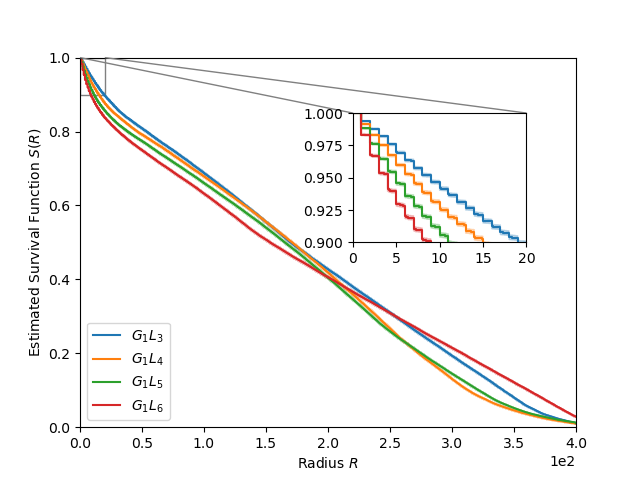
\includegraphics[width=\textwidth]{G_1_initial_radius_sf.png}
          \caption{}
          \label{fig:sf_g1_branch_radius}
        \end{subfigure}
        \hfill
        \begin{subfigure}[b]{0.45\textwidth}
          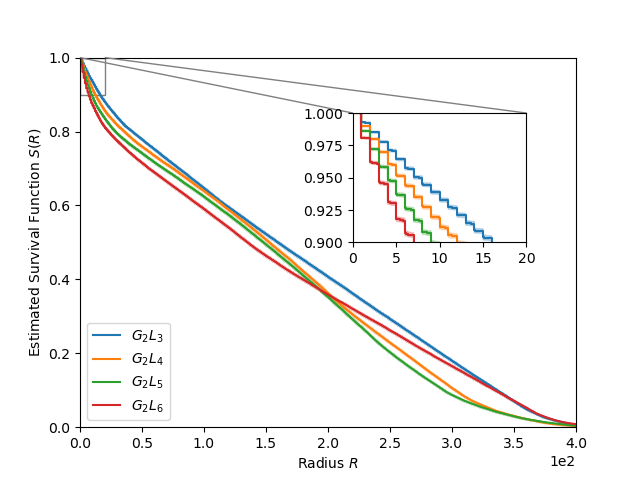
\includegraphics[width=\textwidth]{G_2_initial_radius_sf.png}
          \caption{}
          \label{fig:sf_g2_branch_radius}
        \end{subfigure}

        \caption{}
        \label{fig:sf_branch_radius}

      \end{figure}

      
      \begin{table}
        \centering
        \begin{tabular}{llrrrr}
          \toprule
                       &             &         &  p &    &     \\
          \cmidrule{3-6}
                       &             & Logrank & TW & GB & FH  \\
          \midrule
          $G_1$ $L_3$  & $G_1$ $L_4$  &  0.0 &  0.0 &  0.0 &  0.0     \\
                       & $G_1$ $L_5$  & 0.0 & 0.0 & 0.0 & 0.0    \\
                       & $G_1$ $L_6$  & 0.0 & 0.0 & 0.0 & 0.0      \\
          $G_1$ $L_4$  & $G_1$ $L_5$  & 0.1773 & 0.0 & 0.0 & 0.0      \\
                       & $G_1$ $L_6$  & 0.0 & 0.0 & 0.0 & 0.0       \\
          $G_1$ $L_5$   & $G_1$ $L_6$ & 0.0 &  0.0 & 0.0 & 0.0      \\
          \bottomrule
        \end{tabular}
        \label{tab:g1_ingroup_tests_radius}
        \caption{}
      \end{table}


      \begin{table}
        \centering
        \begin{tabular}{llrrrr}
          \toprule
                       &             &         &  p &    &     \\
          \cmidrule{3-6}
                       &             & Logrank & TW & GB & FH  \\
          \midrule
          $G_2$ $L_3$  & $G_2$ $L_4$  &  0.0 &  0.0 &  0.0 &  0.0     \\
                       & $G_2$ $L_5$  & 0.0 & 0.0 & 0.0 & 0.0    \\
                       & $G_2$ $L_6$  & 0.0 & 0.0 & 0.0 & 0.0      \\
          $G_2$ $L_4$  & $G_2$ $L_5$  & 0.0 & 0.0 & 0.0 & 0.0      \\
                       & $G_2$ $L_6$  & 0.0 & 0.0 & 0.0 & 0.0       \\
          $G_2$ $L_5$   & $G_2$ $L_6$ & 0.0 & 0.0 & 0.0253 & 0.0253      \\
          \bottomrule
        \end{tabular}
        \label{tab:g2_ingroup_tests_radius}
        \caption{}
      \end{table}


      


















    


      \newpage
      
    \subsection{Conclusion}

      \begin{itemize}
         \item In a short time, the survival function of rectangle decays faster than the circle, which conforms to the analytical results.
  
         \item The differences of estimated survival functions between circle and rectangle are statistically significant, which coincides with the real shape dissimilarities.

         \item Within a same group, when $t$ is small, the more branching the object is, the faster the survival function decays.

         \item Within a same group, the pairwise survival functions are statistically different.

         \item The corresponding target structures in $G_1$ and $G_3$ are invariant shapes under translation since their survival function are not statistically different. In other words, periodic boundary conditions of the image can eliminate the effect of the locations.

         \item LRWs can describe and classify the geometries, their spatial configurations, and the unoccupied area in the image.
    \end{itemize}






  % _____________ Section 3: Conclusion ________________________
  %\section{Conclusion}\label{section:branch_conclusion}

...



  
  
%%%%%%%%%%%%%%%%%%%%%%%%%% CHAPTER 4 %%%%%%%%%%%%%%%%%%%%%%%%%%%%%%%%%%
\chapter{LRWs in Real Root Images}

 

%%%%%%%%%%%%%%%%%%%%%%%%%% CHAPTER 5 %%%%%%%%%%%%%%%%%%%%%%%%%%%%%%%%%%
\chapter{Conclusion}
  


  
%%%%%%%%%%%%%%%%%%%%%%%%%% CHAPTER 6 %%%%%%%%%%%%%%%%%%%%%%%%%%%%%%%%%%
\chapter{Future Work}

  %___________ Section 1: Conclusion __________________
  %\section{Conclusion}

...




 




% ___________________________ AFTER BODY OF THESIS _________________________

% 12. Referencing Other Works
  % includes quotations, borrowed thoughts or expression


% 13. Appendices
  \uofsappendix % Activate thesis appendix mode

  \begin{appendices}

    \chapter{Numerical Methods for Solving Parabolic Partial Differential Equations}
      \section{Introduction}

\begin{itemize}
  \item Parabolic PDEs: to characterize time-dependent phenomena
  \item The intrinsically similar features of the traditional computational techniques are mesh discretization in time and space.
\end{itemize}


\section{Summary of Commonly Used Numerical Techniques}

  \subsection{Finite Difference Method (FDM) \cite{grossmann2007numerical}}

  \subsection{Finite Element Method (FEM) \cite{zlamal1968finite}}

  
  \subsection{Other Tranditional Computational Methods}



\section{Limitation in Practice}


    \chapter{Method Validation in Annulus}
      \section{Analytical Results}


\section{Numerical Approximation}



\section{Comparison of Numerical and Analytical Results}


\section{Conclusion}

    
  \end{appendices}
  
  

% 14. Referencing and Bibliography
  % should be arranged either alphabetically or numerically
  \uofsbibliography{thesisref}
  %\bibliographystyle{unsrt}


% 15. Electronic Supplements


\end{document}
